\documentclass{beamer}

%\usetheme{Malmoe}
\usetheme{Szeged}
\usecolortheme{crane}

\newtheorem{remark}{Remark}

\usepackage{listings}
\usepackage{beamerthemesplit}

\lstnewenvironment{newcode}{\lstset{language=Haskell,basicstyle=\scriptsize,escapechar=\@}}{}
\newcommand{\ttcode}[1]{{\color{red}{\tt{#1}}}}

\setbeamertemplate{navigation symbols}{}

\newenvironment{codeblock}[1][.8]{%
\begin{columns}
\begin{column}{#1\linewidth}
\begin{exampleblock}{}}{%
\end{exampleblock}
\end{column}
\end{columns}} 

\newenvironment{execblock}[1][.8]{%
\begin{columns}
\begin{column}{#1\linewidth}
\begin{block}{}}{%
\end{block}
\end{column}
\end{columns}} 

\def\slideskip{\vskip 0.1in}
\def\frameskip{\vskip 0.1in}

\usepackage{hyperref}

\def\@fnsymbol#1{\ensuremath{\ifcase#1\or *\or \dagger\or \ddagger\or
   \mathsection\or \mathparagraph\or \|\or **\or \dagger\dagger
   \or \ddagger\ddagger \else\@ctrerr\fi}}
\renewcommand{\thefootnote}{\fnsymbol{footnote}}   
\newcommand{\forget}[1]{}
\title{{\tt mov} is Turing Complete}
\subtitle{CS4440 Spring 2017}
\author[]{Stephen Dolan\footnote{...as told by Bill Harrison}}
\date{\today}

\begin{document}

\frame{\titlepage}

%%%%%%%%%%%%%%
%%%%%%%%%%%%%%
%%%%%%%%%%%%%%
%%%%%%%%%%%%%%
\section{Introduction}

\begin{itemize}
\item x86 instruction set is, to put it mildly, \emph{complex}
\pause
\item 

\end{itemize}

%%%%%%%%%%%%%%
%%%%%%%%%%%%%%
%%%%%%%%%%%%%%
%%%%%%%%%%%%%%
\section{Machine Model}

\begin{frame}[fragile]
\frametitle{Machine Model}

\begin{itemize}
\item Assume

\begin{center}
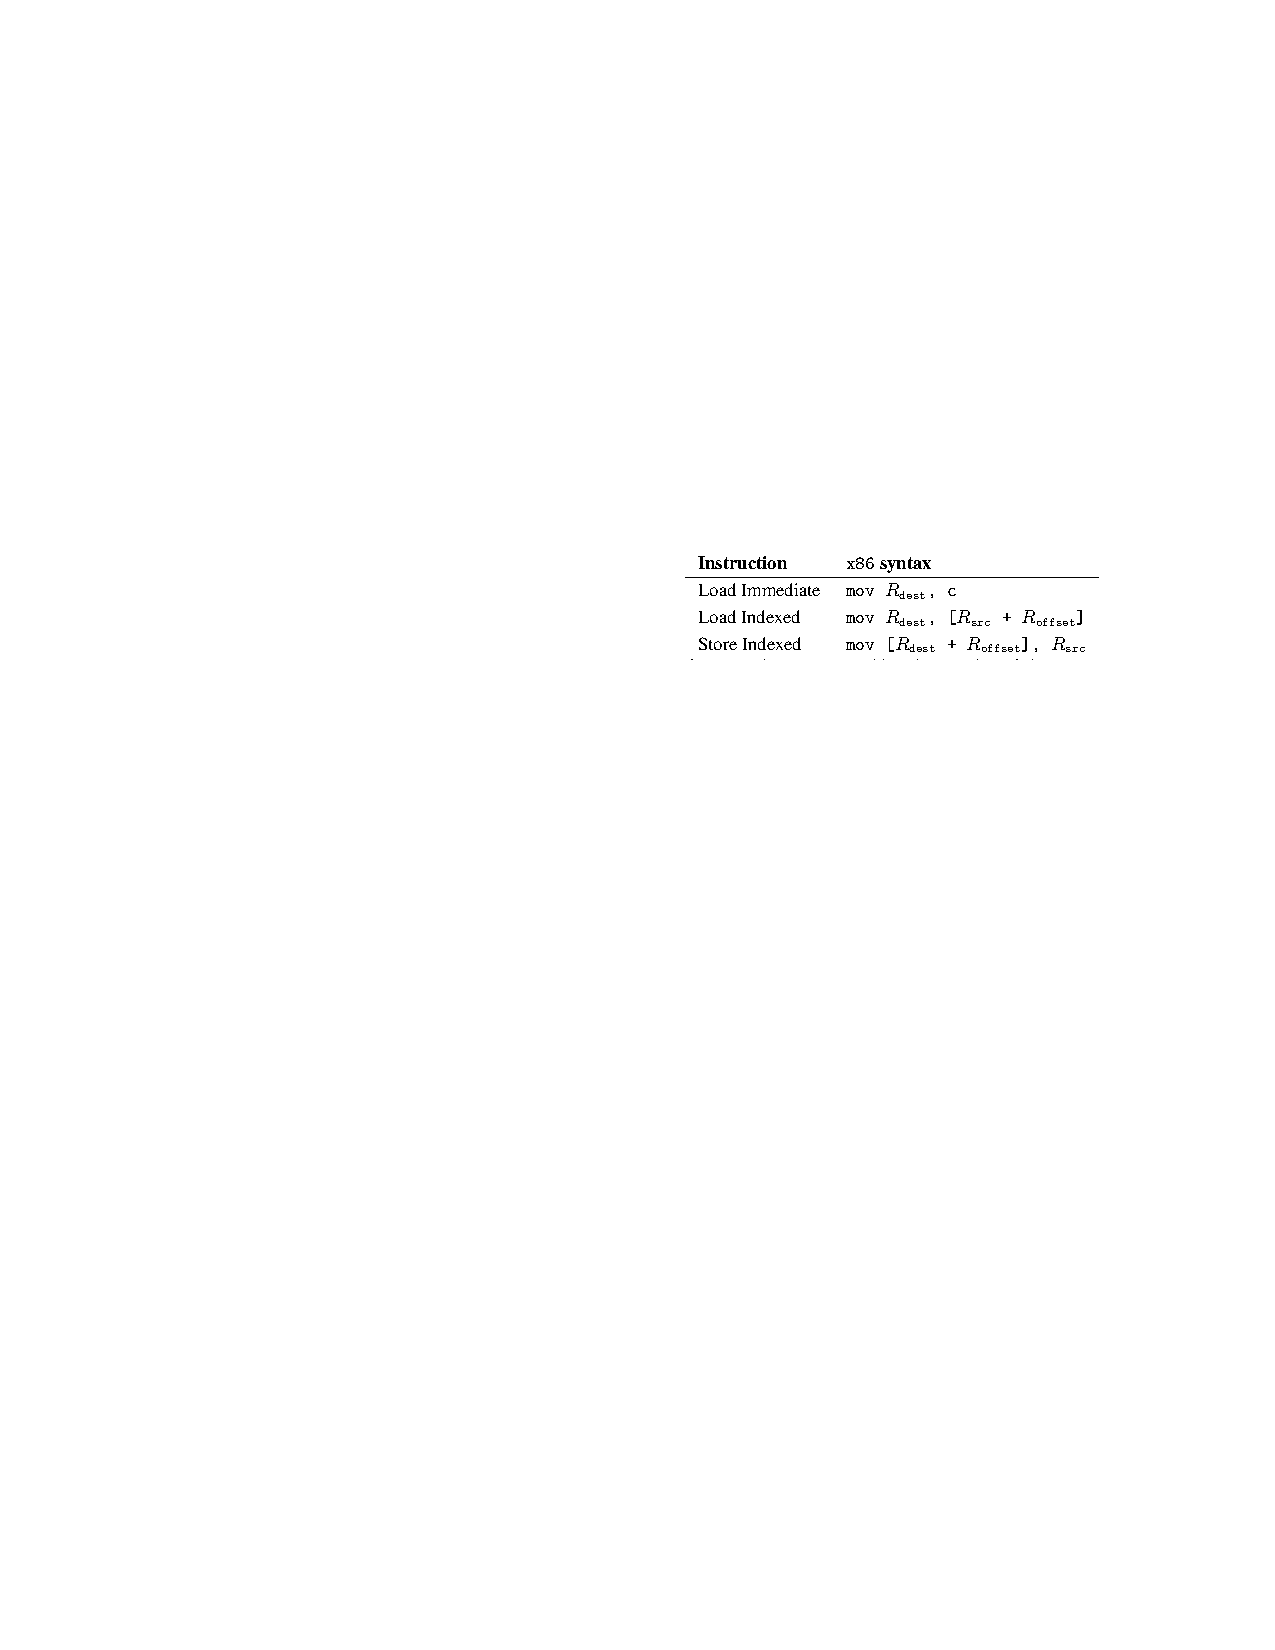
\includegraphics[scale=0.5]{figures/x86instructions}
\end{center}
\end{frame}

%%%%%%%%%%%%%%
%%%%%%%%%%%%%%
%%%%%%%%%%%%%%
%%%%%%%%%%%%%%
\section{Representing Turing Machines}

\begin{frame}[fragile]
\frametitle{Defining Turing Machines}

\begin{center}
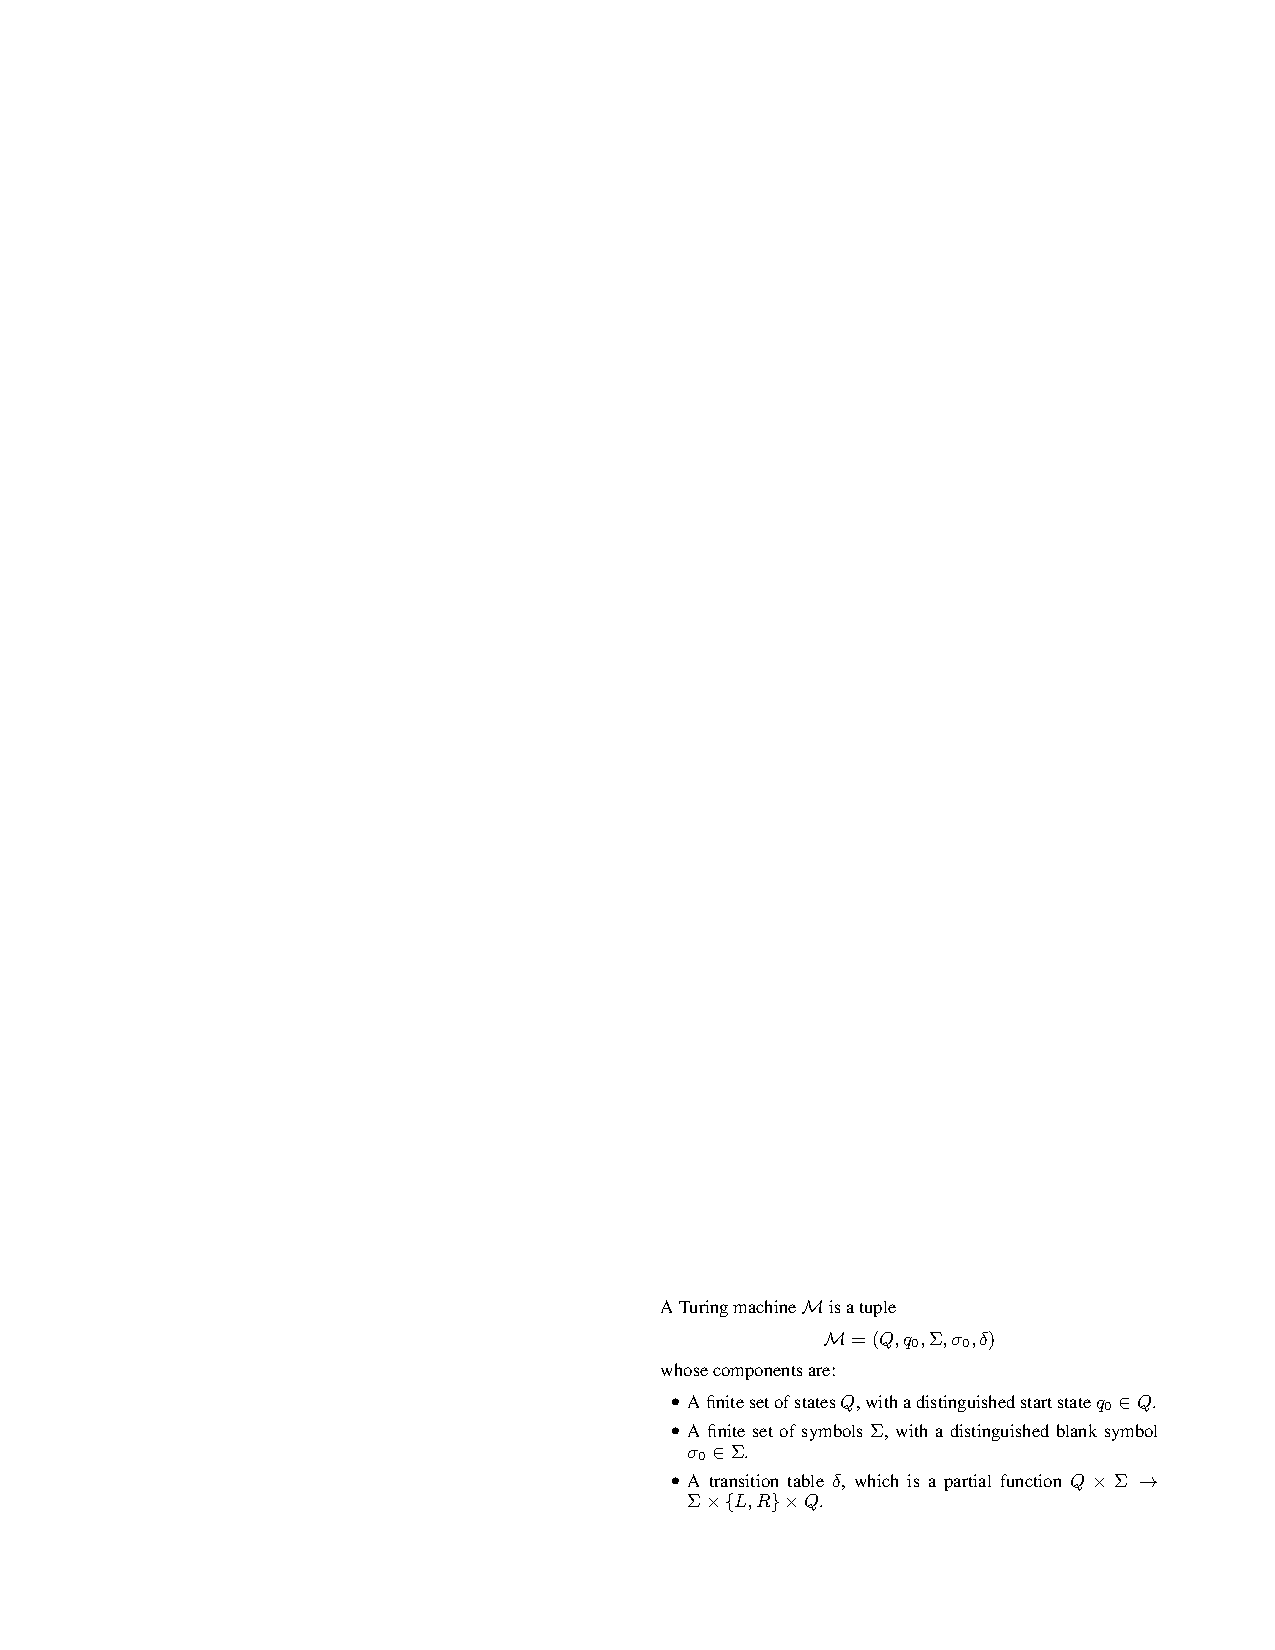
\includegraphics[scale=1.1]{figures/TuringMachine}
\end{center}
\end{frame}


\begin{frame}[fragile]
\frametitle{Representation of a Turing Machine}

\begin{center}
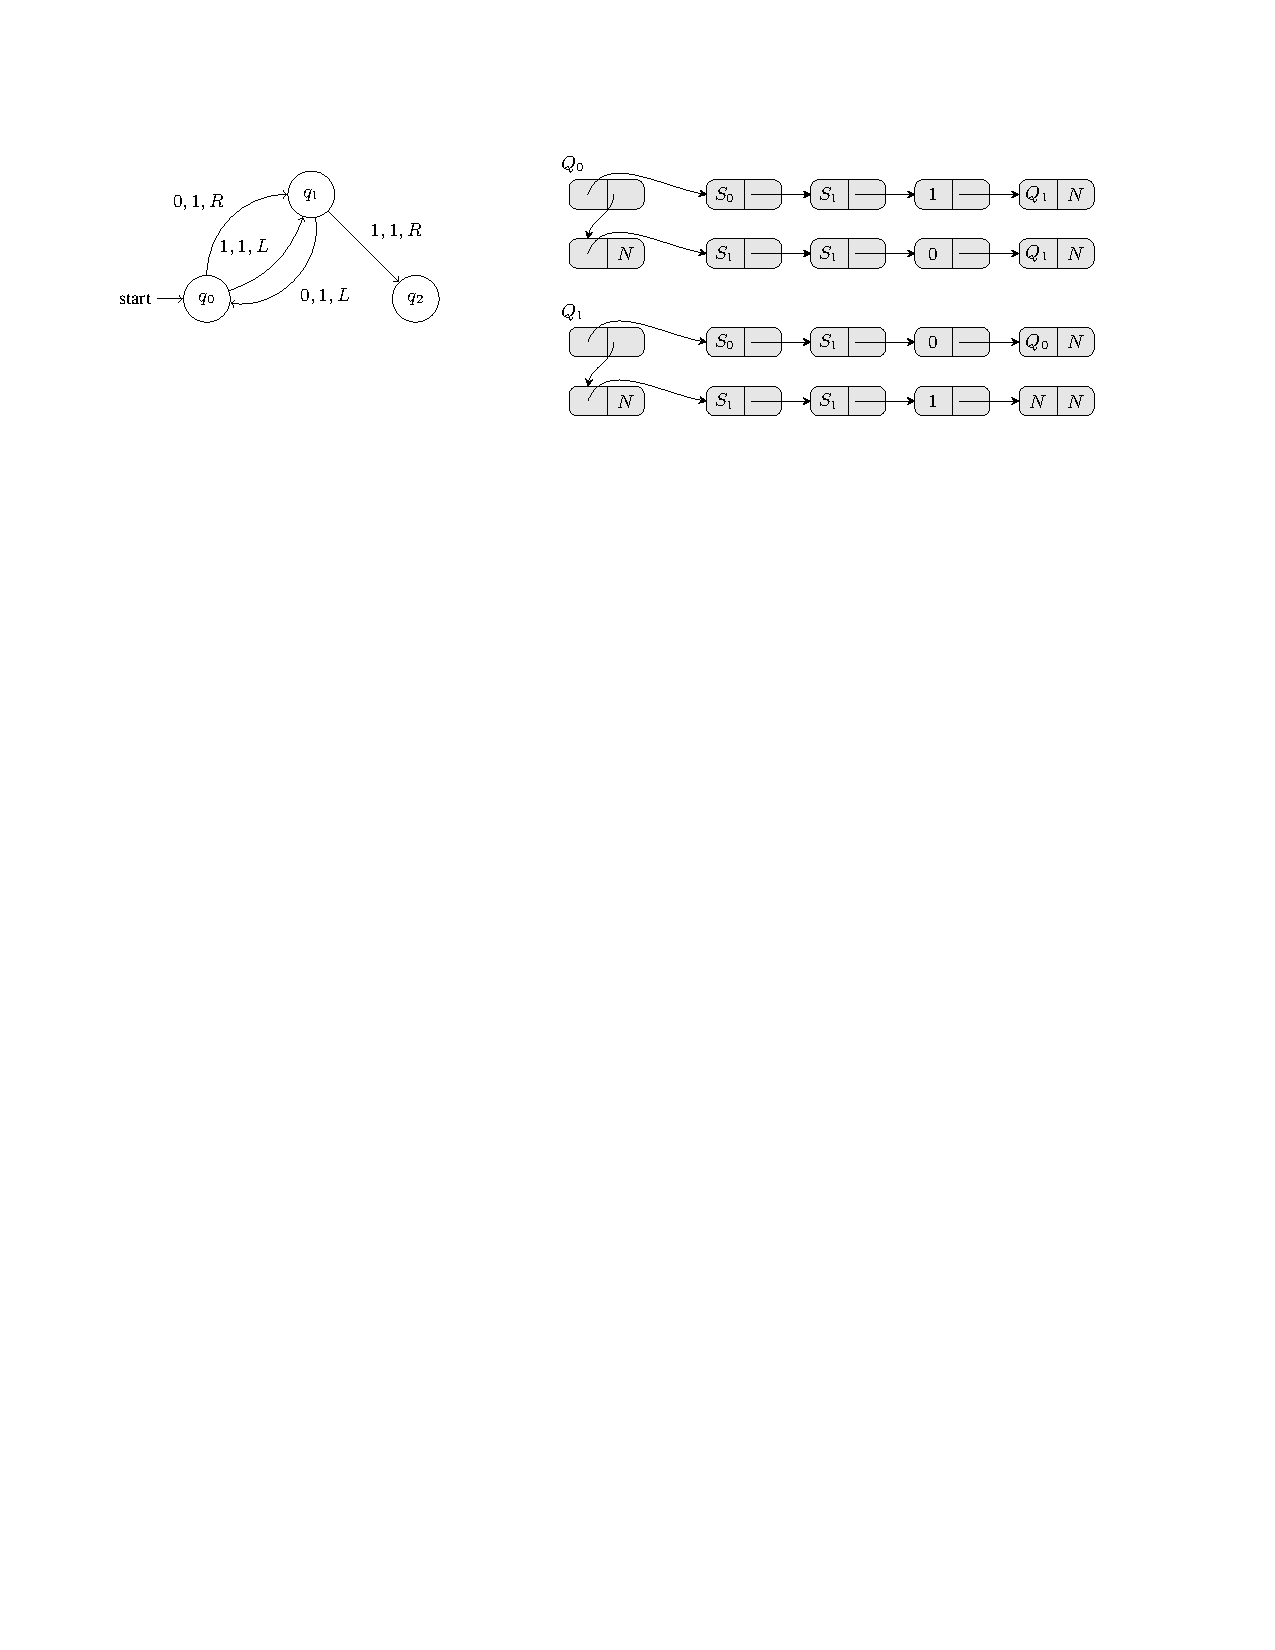
\includegraphics[scale=0.6]{figures/TMrepresentation}
\end{center}
\end{frame}
%%%%%%%%%%%%%%
%%%%%%%%%%%%%%
%%%%%%%%%%%%%%
%%%%%%%%%%%%%%
\section{Comparisons and Conditionals}

%\begin{frame}[fragile]
%\frametitle{}
%
%\begin{center}
%\includegraphics[scale=0.5]{figures/}
%\end{center}
%\end{frame}

%%%%%%%%%%%%%%
%%%%%%%%%%%%%%
%%%%%%%%%%%%%%
%%%%%%%%%%%%%%
\section{Simulating a Turing Machine}

%\begin{frame}[fragile]
%\frametitle{}
%
%\begin{center}
%\includegraphics[scale=0.5]{figures/}
%\end{center}
%\end{frame}

%%%%%%%%%%%%%%
%%%%%%%%%%%%%%
%%%%%%%%%%%%%%
%%%%%%%%%%%%%%
\section{Register Use}

\begin{frame}[fragile]
\frametitle{}

\begin{center}
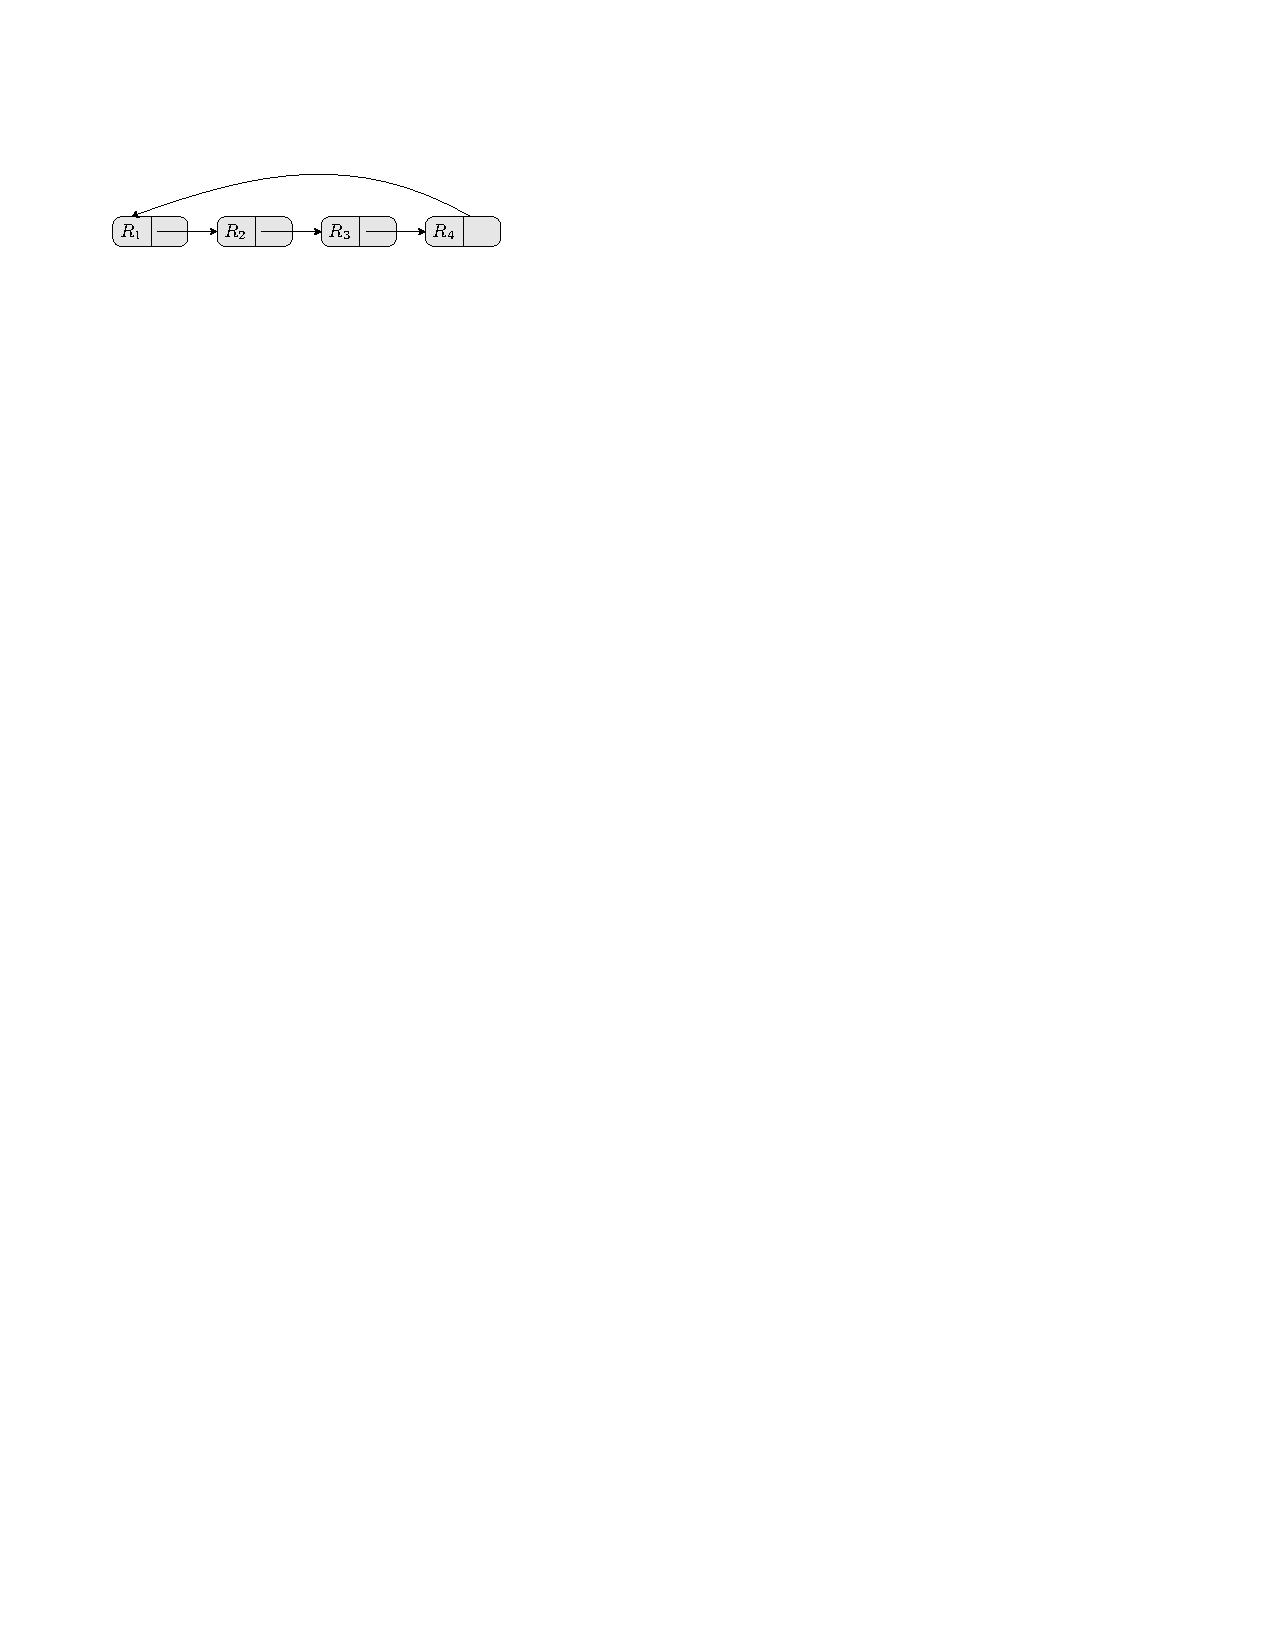
\includegraphics[scale=0.5]{figures/scratchspace}
\end{center}
\end{frame}

%%%%%%%%%%%%%%
%%%%%%%%%%%%%%
%%%%%%%%%%%%%%
%%%%%%%%%%%%%%
\section{Discussion}

%\begin{frame}[fragile]
%\frametitle{}
%
%\begin{center}
%\includegraphics[scale=0.5]{figures/}
%\end{center}
%\end{frame}



\end{document}
    
